\documentclass[a4paper,11pt,fleqn]{article}%fleqn pour aligner les equations à gauche

\usepackage{../../Styles/Exercice}

\newcommand{\chnum}{Chapitre 02}
\newcommand{\chtitle}{Composition Chimique des Solutions}
\newcommand{\dtype}{Exercices}

\begin{document}
	\maketitle
\begin{multicols}{2}
    \section{La bouteille bleue}
    La bouteille bleue est une expérience au cours de laquelle la solution à l'intérieur de la bouteille change de couleur quand on l'agite.\\
    L'espèce chimique responsable de la coloration de la bouteille est le bleu de méthylène. Au repos, le bleu de méthylène réagit avec du glucose dissous et est présent sous sa forme incolore. Lors de l'agitation, le bleu de méthylène réagit avec le diioxygène de l'air pour se transformer dans sa forme colorée. Une fois l'agitation terminée, le cycle reprend, le bleu de méthylène réagit avec le glucose et la solution se décolore. Et ainsi de suite.\\
    Le spectre d'absorption ci-après est celui du bleu de méthylène.

    \section{Dosage par étalonnage des ions nitrate}
    Les ions nitrate \ce{NO3^-} sont des polluants courants des eaux de surface : une eau contenant plus de \SI{50}{mg.L^{-1}} d'ions nitrate n'est pas potable. Une solution aqueuse d'ions nitrate est incolore, mais prend une coloration jaune en présence d'acide phénoldisulfonique.\\
    On dispose d'une solution aqueuses d'ions nitrate en présence de cet acide, de concentration $c_0 = \SI{1,0E-3}{\mole\per\liter}$. Par dilution, on prépare une échelle de teintes et on mesure les absorbances à \SI{410}{nm}, dans une cuve de largeur $l = \SI{1,0}{cm}$. On obtient les résultats suivants :
    \begin{center}
        \begin{tabular}{|c|c|c|c|c|c|}
            \hline
            $c$ (\si{\mole\per\liter}) & \num{1,0E-3} & \num{7,5E-4} & \num{5,0E-4} & \num{2,5E-4} & \num{1,0E-4} \\
            \hline
            $A$ & 0,95 & 0,67 & 0,47 & 0,23 & 0,1 \\
            \hline
        \end{tabular}
    \end{center}
    \begin{enumerate}
        \item \begin{enumerate}
            \item Tracer le graphique d'étalonnage et la droite moyenne.
            \item Déterminer la valeur du coefficient directeur $k$ de cette droite.
            \item En déduire le coefficient d'absorption molaire $\varepsilon$ des ions nitrate à \SI{410}{nm}.
        \end{enumerate} 
        \item Une eau de rivière est testée dans les mêmes conditions : son absorbance est $A = 0,85$. Déterminer sa concentration en ions nitrate.
        \item Cette eau doit-elle être déclarée non-potable ?
    \end{enumerate}

\section{Relation à l'équivalence}
    On considère le titrage de l'éthanol \ce{C2H5OH} par les ions dichromate \ce{Cr2O7^{2-}} en présence de \ce{H+} en excès. La réaction chimique modélisant ce titrage est :
    \ce{3 C2H5OH + 2 Cr2O7^{2-} + 16 H+ -> 3 CH3COOH + 4 Cr^{3+} + 11 H2O}
    Un elève a tracé le tableau d'avancement suivant :
    \begin{center}
        \begin{tabular}{|m{.3\linewidth}|c|c|c|c|}
            \hline
            Réaction & \ce{C2H5OH} & \ce{Cr2O7^{2-}} & \ce{H+} & $\rightarrow$\\
            \hline
            Quantités de matière de ... & \ce{C2H5OH} & \ce{Cr2O7^{2-}} & \ce{H+} &  \\
            \hline
            ... apportées à l'équivalence & $c\cdot V_{eq}$ & $n_0$ & Excès &  \\
            \hline
            ... présentes à l'équivalence &   &   & Excès &  \\
            \hline
        \end{tabular}
    \end{center}
    \begin{enumerate}
        \item Identifier les notations désignant la quantité de matière d'éthanol introduit, la concentration de la solution titrante et le volume équivalent.
        \item Recopier ce tableau et compléter sa dernière ligne en utilisant la définition de l'équivalence.
        \item En déduire l'expression de la quantité de matière initiale en réactif titré.
    \end{enumerate}

\section{Titrage et graphiques}
On reprend le titrage de l'exercice précédent. Le graphique suivant représente les quantités de matière de \ce{Cr2O7^{2-}} et de \ce{C2H5OH} dans le mélange réactionnel en fonction du volume $V$ de solution titrante versée.
\begin{center}
    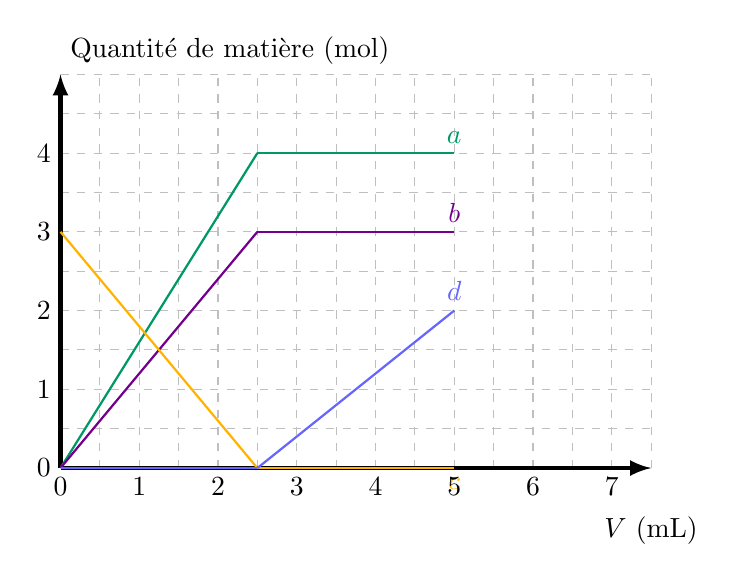
\begin{tikzpicture}
        \draw[gray!50,dashed](0,0) grid[step=.5] (7.5,5);
        \draw[-latex, ultra thick] (0,0) -- (7.5,0);
        \draw[-latex, ultra thick] (0,0) -- (0,5);

        \draw[green!60!blue, thick] (0,0) -- (2.5,4);
        \draw[green!60!blue, thick] (2.5,4) -- (5,4);
        \node[above,green!60!blue] at (5,4) {$a$};

        \draw[purple!60!blue, thick] (0,0) -- (2.5,3);
        \draw[purple!60!blue, thick] (2.5,3) -- (5,3);
        \node[above,purple!60!blue] at (5,3) {$b$};

        \draw[orange!60!yellow, thick] (0,3) -- (2.5,0);
        \draw[orange!60!yellow, thick] (2.5,0) -- (5,0);
        \node[below,orange!60!yellow] at (5,0) {$c$};

        \draw[blue!60!white, thick] (0,0) -- (2.5,0);
        \draw[blue!60!white, thick] (2.5,0) -- (5,2);
        \node[above,blue!60!white] at (5,2) {$d$};

        \foreach \x in {0,1,2,3,4,5,6,7}
            \node[below] at (\x,0) {\x};
        \foreach \y in {0,1,2,3,4}
            \node[left] at (0,\y) {\y};

        \node[below] at (7.5,-.5) {$V$ (mL)};
        \node[above right] at (0,5) {Quantité de matière (mol)};
    \end{tikzpicture}
\end{center}
\begin{enumerate}
    \item Identifier chaque courbe, en justifiant.
    \item Détermine rle volume équivalent $V_{eq}$, la quantité de matière initiale $n_0$ de réactif et la concentration $c$ de la solution titrante.
\end{enumerate}

\section{Titrage et incertitudes}
Lors d'une séance de travaux pratiques, des élèves ont effectué un titrage. Les valeurs des volumes équivalents $V_{eq}$ obtenus par chaque groupe sont les suivantes :
\begin{center}
    \begin{tabular}{|c|c|c|c|c|c|}
        \hline
        \multirow{3}{*}{$V_{eq}$ (mL)} & 13,2 & 13,1 & 12,8 & 12,9 & 13,5 \\
        \cline{2-6}
         & 13,0 & 13,2 & 13,3 & 13,2 & 13,0 \\
        \cline{2-6}
         & 12,9 & 13,6 & 13,6 & 13,3 & 13,2 \\
        \hline
    \end{tabular}
\end{center}
\end{multicols}
\end{document}
